\chapter{Title}\label{chapter: 2}
\section{Theorem Environment}
\begin{theorem}\label{theorem: convergence}
    Let $X_1,X_2,\dots$ be pairwise independent identically distributed random variables with $EX_i<\infty$. Let $EX_i=\mu$ and $S_n=X_1+\cdots+X_n$. Then $S_n/n\rightarrow\mu$ a.s. as $n\rightarrow\infty$.
\end{theorem}

\begin{lemma}\label{lemma: convergence}
    Let $X_1,X_2,\dots$ be pairwise independent identically distributed random variables with $EX_i<\infty$. Let $EX_i=\mu$ and $S_n=X_1+\cdots+X_n$. Then $S_n/n\rightarrow\mu$ a.s. as $n\rightarrow\infty$.
\end{lemma}

\begin{definition}\label{definition: convergence}
    Let $X_1,X_2,\dots$ be pairwise independent identically distributed random variables with $EX_i<\infty$. Let $EX_i=\mu$ and $S_n=X_1+\cdots+X_n$. Then $S_n/n\rightarrow\mu$ a.s. as $n\rightarrow\infty$.
\end{definition}

\begin{proposition}\label{proposition: convergence}
    Let $X_1,X_2,\dots$ be pairwise independent identically distributed random variables with $EX_i<\infty$. Let $EX_i=\mu$ and $S_n=X_1+\cdots+X_n$. Then $S_n/n\rightarrow\mu$ a.s. as $n\rightarrow\infty$.
\end{proposition}

\begin{assumption}\label{assumption: convergence}
    Let $X_1,X_2,\dots$ be pairwise independent identically distributed random variables with $EX_i<\infty$. Let $EX_i=\mu$ and $S_n=X_1+\cdots+X_n$. Then $S_n/n\rightarrow\mu$ a.s. as $n\rightarrow\infty$.
\end{assumption}

\begin{remark}\label{remark: convergence}
    Let $X_1,X_2,\dots$ be pairwise independent identically distributed random variables with $EX_i<\infty$. Let $EX_i=\mu$ and $S_n=X_1+\cdots+X_n$. Then $S_n/n\rightarrow\mu$ a.s. as $n\rightarrow\infty$.
\end{remark}

\begin{corollary}\label{corollary: convergence}
    Let $X_1,X_2,\dots$ be pairwise independent identically distributed random variables with $EX_i<\infty$. Let $EX_i=\mu$ and $S_n=X_1+\cdots+X_n$. Then $S_n/n\rightarrow\mu$ a.s. as $n\rightarrow\infty$.
\end{corollary}

\begin{example}\label{example: convergence}
    Let $X_1,X_2,\dots$ be pairwise independent identically distributed random variables with $EX_i<\infty$. Let $EX_i=\mu$ and $S_n=X_1+\cdots+X_n$. Then $S_n/n\rightarrow\mu$ a.s. as $n\rightarrow\infty$.
\end{example}

\begin{proof}[Proof of Theorem \ref{theorem: convergence}]
    Proof of the theorem.
\end{proof}

\section{Enumerate}

\begin{itemize}
    \item a.
    \item b.
\end{itemize}

\begin{enumerate}
    \item 1.
    \item 2.
\end{enumerate}

\begin{enumerate}[(1)]
    \item (1).
    \item (1).
\end{enumerate}

\begin{enumerate}[(a)]
    \item 1
    \item 2
\end{enumerate}

\section{Algorithm}
\begin{algorithm}[htb]
    \SetAlgoLined
    {\bf Initialization:} $S=\varnothing$.
        
    \For{$i=1,\ldots,N$}{
    Generate a Bernoulli variable $R_i\sim\text{Bernoulli}(p_i)$\;
    \If {$R_i=1$}{ Update $S=S\cup\{(\bm {x}_{i},y_{i},p_{i})\}$.}{}
    }
    {\bf Estimation:} Obtain  $\hat{\bm\beta}_{sub}$ by maximizing the following weighted likelihood function  based on the subsample $S$.
    \caption{General Poisson subsampling algorithm}
    \label{algorithm: poisson subsampling}
\end{algorithm}

\section{Table}

\begin{table}[htb]
    \caption{\normalsize Caption.}
    \centering
    \begin{threeparttable}
    \setlength{\tabcolsep}{23mm}{ % 控制表格长度
    \begin{tabular}{lll}
        \hline
        Col~1 & Col~2 & Col~3 \\
        \hline
        1.98 & 2.14 & 4.15 \\
        2.18 & 1.90 & 1.45 \\
        \hline
    \end{tabular}}
    \begin{tablenotes}[para,flushleft]
        \footnotesize{footnote}
    \end{tablenotes}
    \end{threeparttable}
    \label{table: label}
\end{table}


\section{Figure}

\begin{figure}[htb]
    \centering
    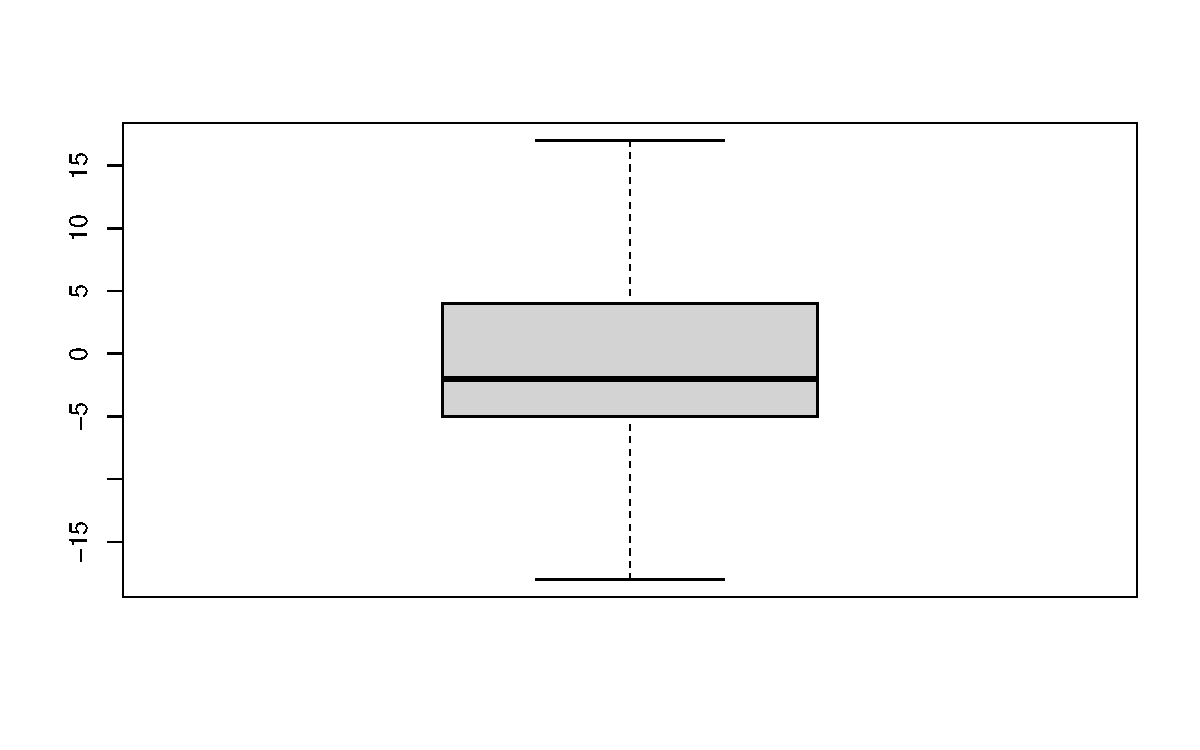
\includegraphics[width=0.95\textwidth]{boxplot}
    \caption{Caption}
    \label{figure: 1}
\end{figure}

\begin{figure}[htp]
    \centering
    \begin{subfigure}{0.49\textwidth}
      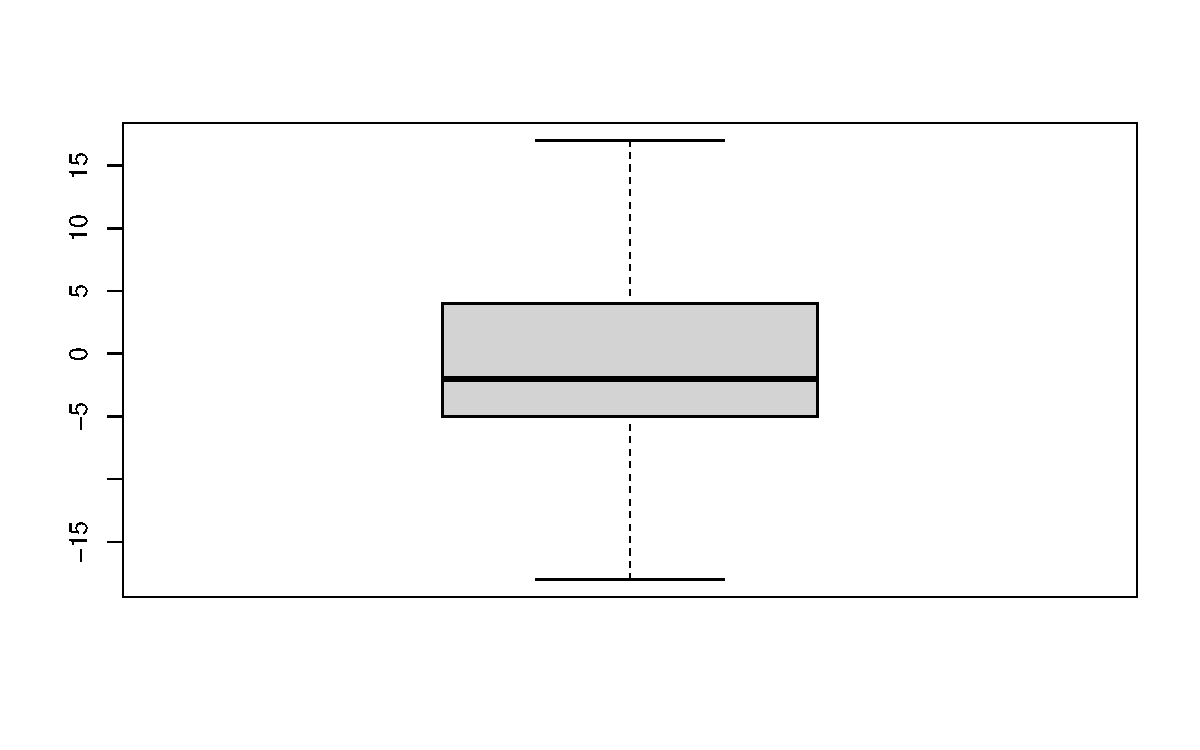
\includegraphics[width=\textwidth]{boxplot}
      \caption{1.}
    \end{subfigure}
    \begin{subfigure}{0.49\textwidth}
      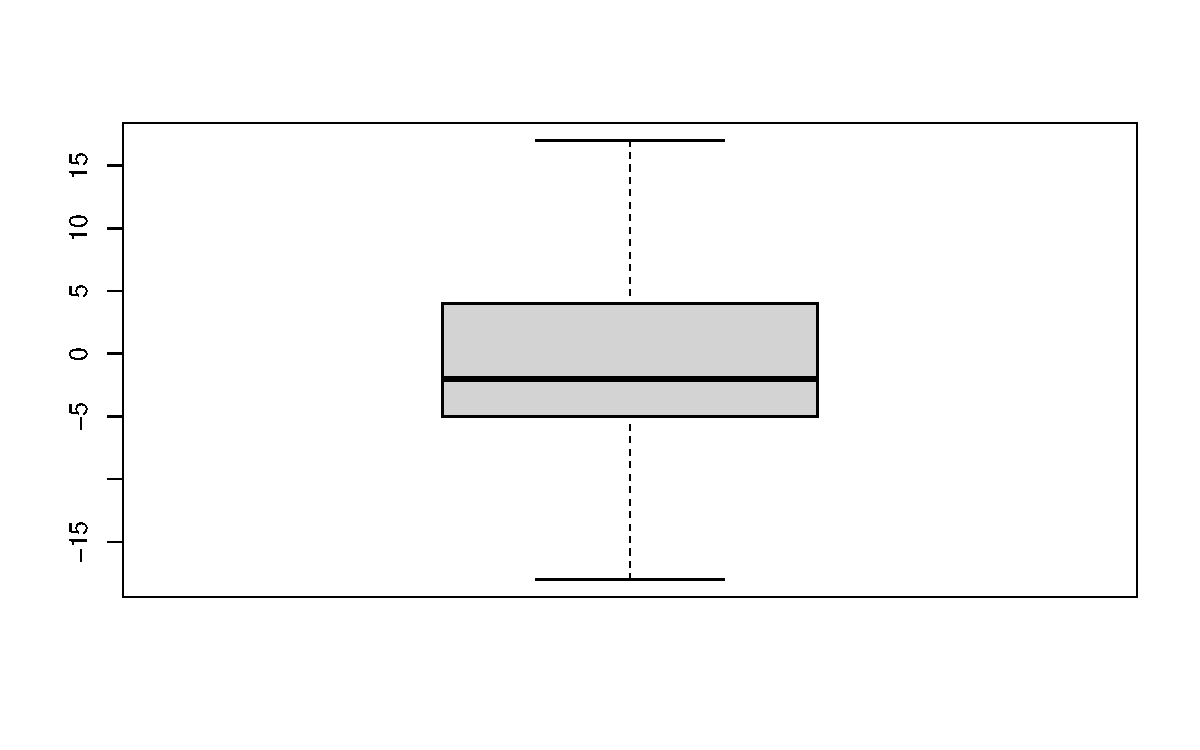
\includegraphics[width=\textwidth]{boxplot}
      \caption{2.}
    \end{subfigure}
    \caption{Caption}
    \label{figure: 2}
\end{figure}
  
\begin{figure}[htb]
    \centering
    \begin{subfigure}{0.49\textwidth}
      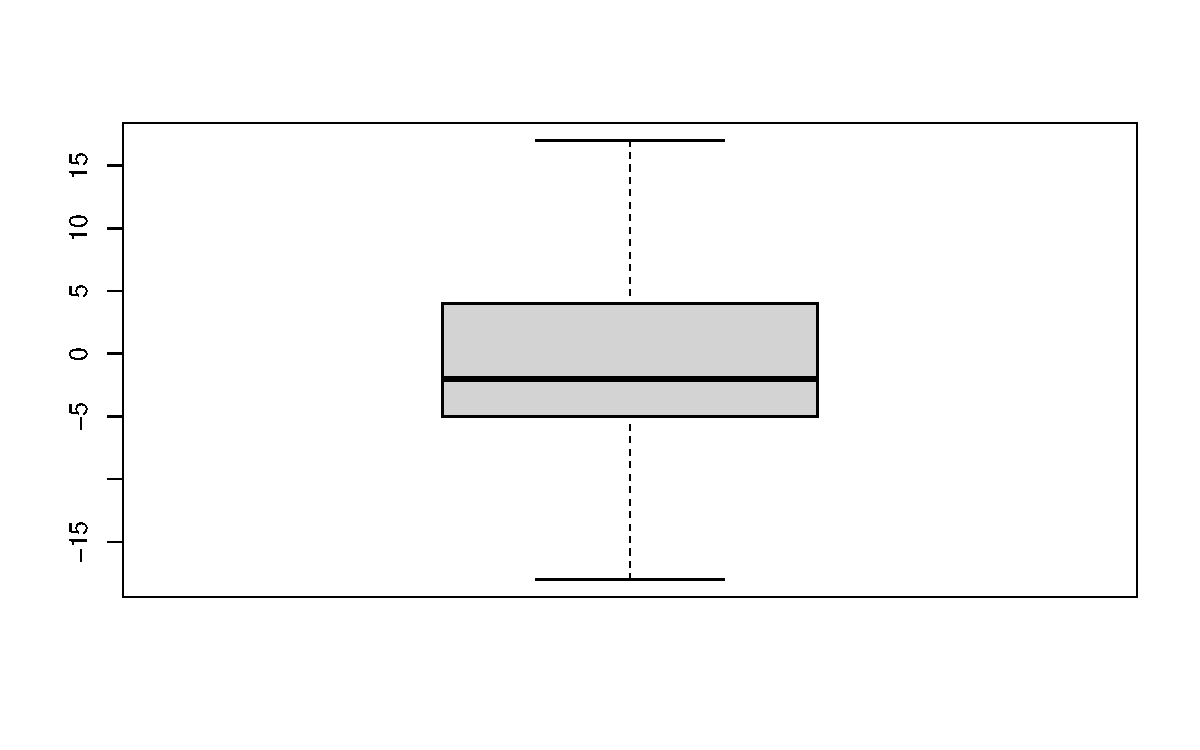
\includegraphics[width=\textwidth]{boxplot}
      \caption{1.}
    \end{subfigure}
    \begin{subfigure}{0.49\textwidth}
      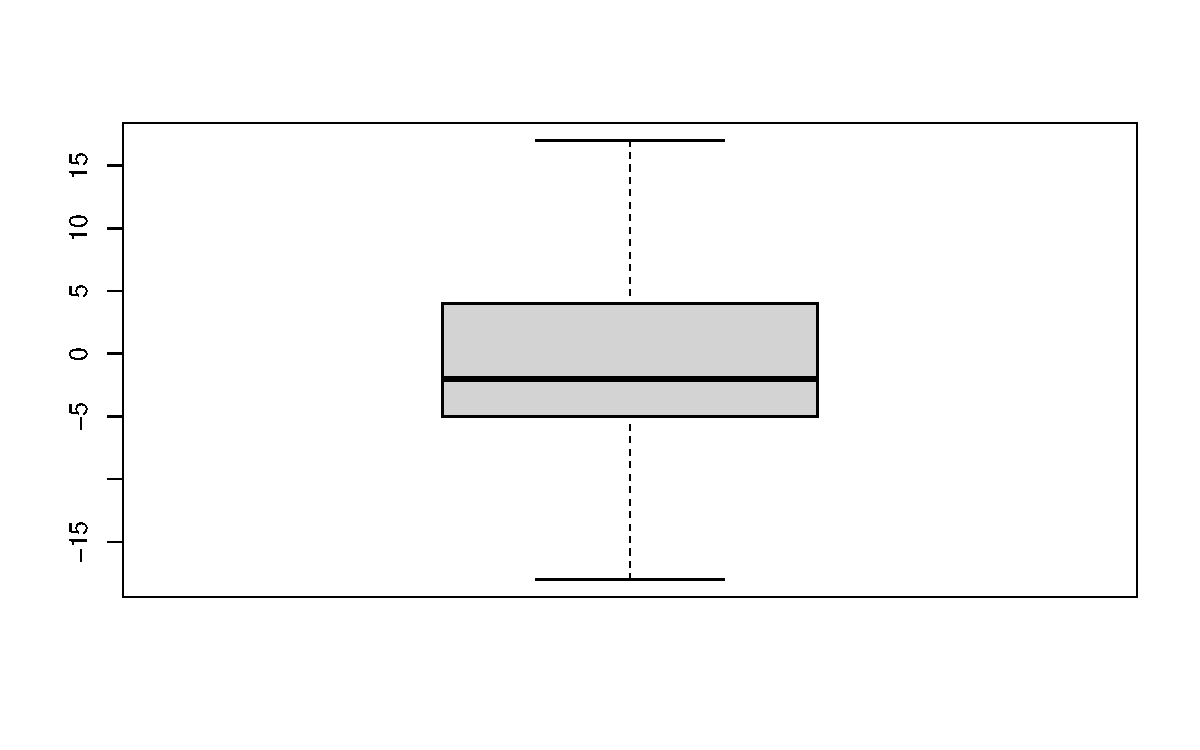
\includegraphics[width=\textwidth]{boxplot}
      \caption{2.}
    \end{subfigure}\\[1mm]
    \begin{subfigure}{0.49\textwidth}
      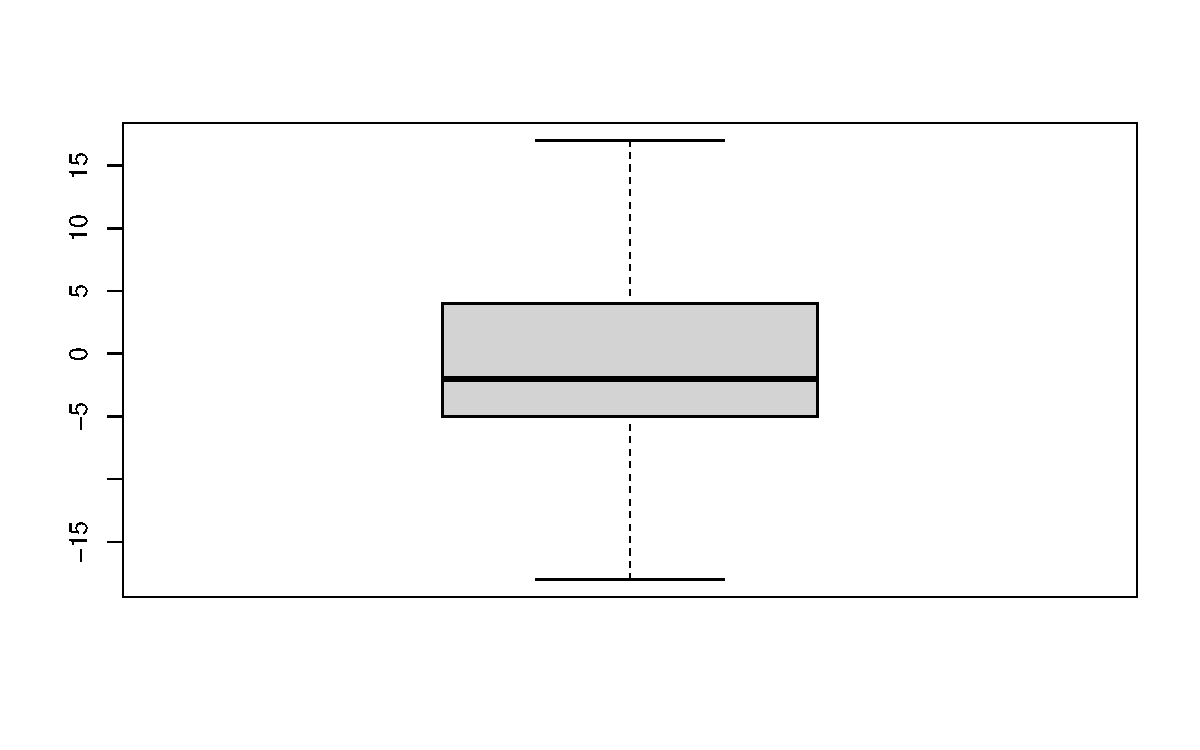
\includegraphics[width=\textwidth]{boxplot}
      \caption{3.}
    \end{subfigure}
    \begin{subfigure}{0.49\textwidth}
      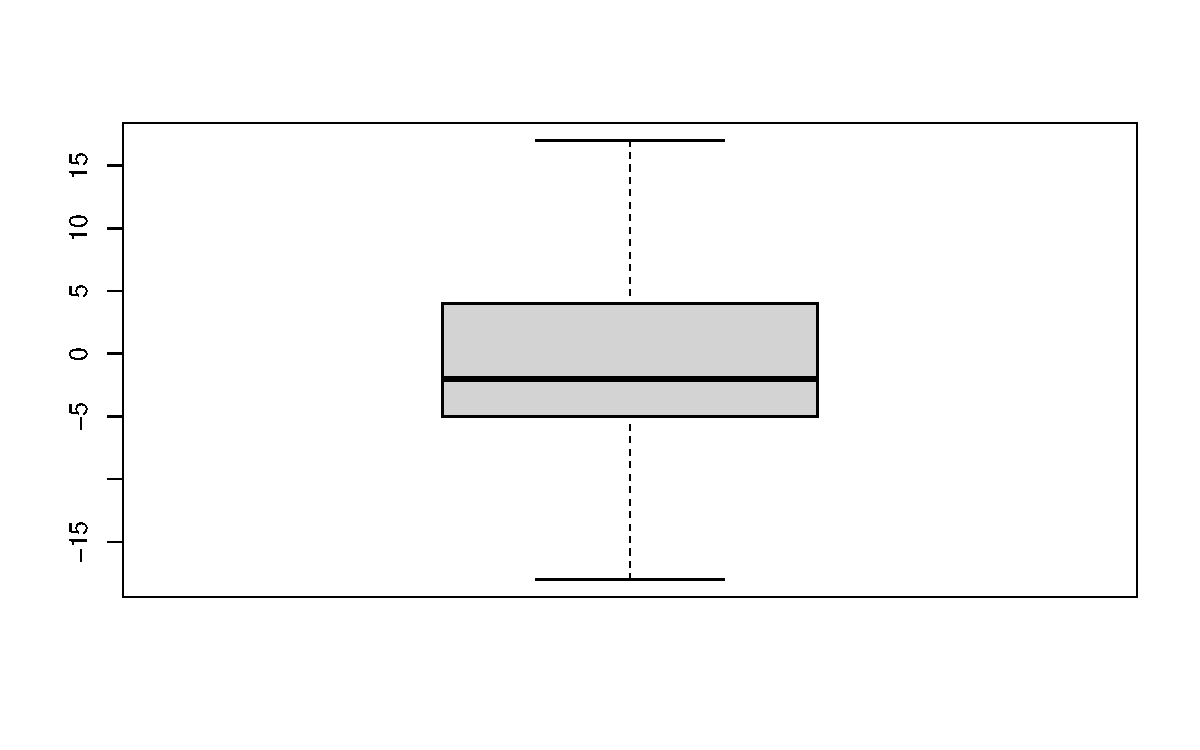
\includegraphics[width=\textwidth]{boxplot}
      \caption{4.}
    \end{subfigure}\\[1mm]
    \caption{Figure.}
    \label{figure: 3}
\end{figure}

\section{Add References}
\cite{xue2020online}. \citep{xue2020online}
